\documentclass[a4paper,12pt]{article}
\usepackage{color}
\usepackage{graphicx}
\usepackage{listings}

\usepackage{hyperref}

\usepackage{float}

\begin{document}

\title{Bhargava Design Handbook}
\author{Aman Bhargava}
\date{\today}
\maketitle

\tableofcontents

\section{Identity}
\subsection{A Brief Biography}
My name is Aman Bhargava, and I am currently an Engineering Science student at the University of Toronto. I was born and raised in the state of Maine in the United States, and I moved to Cobourg, Ontario when I was 12.

\subsection{My Values}
I value altruism, creativity/open-mindedness, efficiency, and practicality. Figure 1 represents the flowchart of goodness I see these forming.

\begin{figure}[H]
\centering
\includegraphics[width=0.9\textwidth]{img/image001.png}
\caption{How my values integrate with the steps to my goal of significantly and positively changing the world.}
\label{}
\end{figure}

I believe that this general cycle has the power to have a significant and positive effect on the world, which is one of my most deeply-held ambitions in life.

\subsection{Skills}
\begin{enumerate}
\item Team organization and leadership: Through my experience in leading group projects in school, university, hackathons and more, I have learned how to run an effective, goal-driven team.
\item Programming: I have confidence in my ability to implement ideas into software, at least in such a way that can communicate a basic idea.
\item Data Analysis: I am competent with data visualization, basic statistics, supervised machine learning, and basic clustering.
\item Fabrication: I am competent with basic fabrication tools, namely those found in the Light Fabrication Facility (3D-printing, laser cutting, foam core, basic carpentry, arduino/raspberry pi programming)
\item Argumentation: As a former provincial debater, I believe in my ability to effectively use argumentation to get closer to the truth in the vast majority of issues that I am able to understand.
\item Research: I am able to effectively utilize engineering and scholarly libraries and databases to get the information that I need.
\item Self-learning: My ability to learn things as needed on my own has proven useful time and time again in all of my projects.
\end{enumerate}

\subsection{Biases}
Everything I have written so far in this introduction is a potential bias. Due to my experience in programming, I am likely overly willing to go down the technological route to solve problems without considering non-technological solutions. Because I pride myself in my ability to teach myself, I am less likely than would be optimal to ask for help or consider the possibility of a project being out of my abilities.

Beyond the biases I have implicitly defined in this introduction, I think that my personality makes me overly willing to go outside the box for projects. Because I value creativity so highly, I find it boring to go by the book and am susceptible to the temptation of going outside the box even when it might not be favourable for the design objective.

More generally, I am biased by what I think is “boring” and “interesting”. Even when I try not to, one of the first things I think of when I consider a design alternative or process idea is how “cool” it seems. Even if an alternative will meet the needs of our requirements model/our stakeholders’ needs, I will be turned off of it if it doesn’t meet my subjective, unconscious criteria for what is “interesting”.

Finally, I have been in private schools for my entire life. Simultaneously, I have frequently visited my parent’s home country of India, where I have been exposed (for several weeks at a time) to extreme poverty. I have most of my time around two ends of the socio-economic spectrum, and I am almost certainly biased by that extremism, though I find it difficult to predict exactly how.

\subsection{Metadiscourse on Handbook Design}
I will go on to discuss my projects, including the process followed and holistic review for each, followed by a description and justification of my personal design process, and finally a full overview of all the tools, models, and frameworks mentioned and briefly discussed in the projects section.

My handbook is organized this way because my projects are a core part of my identity and therefore ought to be introduced first to better understand my use of tools and the derivation of my personal design process. I choose to be detailed about my projects because, in my experience in writing guides for my future self, I require many mental hooks to draw upon in order to recall concepts, ideas, and skills optimally.

This organization also mirrors my value system organization. I introduce my projects (i.e. ‘identifying worthy problems to solve’), then my personal design process (i.e. a tool to ‘generate creative, good solutions to these problems’), and finally close with detailed description of each engineering design tool (i.e. methods to ‘optimize my plan and effectively implement the great ideas’).

I chose not to group my Tools into categories such as FDCR because I invented many of them and many are from outside of Praxis lectures, so they don’t fit directly into easily describable categories. As well, when I am looking through in the future, being forced to look through all my favourite tools will help me to potentially creatively alter a tool that wouldn’t initially fit the use case, but could both my project via its effectiveness and actualize my values of creativity and open mindedness.

My invented tools are valid because I have evidence in the form of my experience that they work for me. Since this handbook is meant for my future design work, I am a key stakeholder and that it plenty of reason to be valid. On top of this, I incorporate further research to justify why many of my invented tools are valid.




\section{Projects}
\subsection{Importance of Projects}
I have always been a project-oriented person, and I love doing projects. Using projects as case studies has been extremely valuable for my success in later projects. The following is a brief summation of some of my projects from the past year, since the beginning of Praxis I. I will present them in chronological order, discussing the project goals, process, and a brief holistic review.

\subsection{Praxis I Design - Smart Hat}
\label{sec:hat}
For our Praxis I design project, Alice, Kelvin and I worked to improve the quality of sleep for Engsci’s in transit. We designed for effectiveness in terms of light and sound blockage, along with cost, comfort, durability, and aesthetics.

\subsubsection{Process}
We diverged a multitude of ideas using tools such as \textbf{extreme DfX} (\ref{sec:extreme}) and then converged to a conceptual design via \textbf{system 1.5 analysis} and comparing our alternatives using high-level objectives via \textbf{logical argumentation and research}. We built a low-fidelity prototype using a Santa hat and a pair of cheap headphones to demonstrate our idea and to get a sense of the scale. Then, we used the \textbf{divide and conquer} (\ref{sec:conquer}) design tool to divide our design exercise into many smaller design problems and did smaller rounds of framing, diverging, and converging for each detailed design decision. This enabled us to turn our conceptual design into a detailed, well-substantiated design.

\begin{figure}[H]
\centering
\includegraphics[width=1\textwidth]{img/image002.jpg}
\caption{Demonstrating beta prototype. Our final design retained the shape presented but used \textbf{divide and conquer} (\ref{sec:conquer}) to add rigour to the fine details.}
\label{}
\end{figure}

\begin{figure}[H]
\centering
\includegraphics[width=1\textwidth]{img/image003.jpg}
\caption{Our final design, post divide and conquer. The design is far more specific and rigorous than the beta version, but is remains informed by the initial design.}
\label{}
\end{figure}

\subsubsection{Holistic Review}
Overall, I believe that we made a well-argued case for our design. We had comprehensive research and strong prototyping, but I believe that we were rather held back by our attachment to dogmatic design. We were concerned more about the quality of our grades rather than the quality of our designs. Because of this, we were overly attached to the design process discussed in class. We initially did not realize that we were allowed to break our design decision into multiple smaller design decisions. Because of this, we thought that we would need to go through a tremendous number of fully-fledged alternatives in order to arrive at a ‘well justified’ final design. It was only after I drafted this alternative journey 3 days before the due date that we were able to really move forward well.

The biggest lesson learned was that the design process is malleable. If one can come up with a good reason to change the design process to better fit the opportunity at hand, it is their duty as an engineer to at least argue for that change in the design process.

\begin{figure}[H]
\centering
\includegraphics[width=0.9\textwidth]{img/image004.jpg}
\caption{My initial proposal for the group to use the 'divide and conquer' method to finalize our design. The experience of changing the design process influenced the rest of my projects and my personal design process profoundly.}
\label{}
\end{figure}


\subsection{CIV102 - Genetic Bridge Algorithm}
\label{sec:bridge}
The CIV102 bridge project is a staple of Engsci, but my biggest takeaway from it was a ‘side project’ of sorts that stemmed from the main project. We were tasked with making a matboard bridge that could hold the maximum amount of weight under some specified loading conditions. In class, we learned the formulae that would give the amount of weight a bridge would hold before failing by some arbitrary failure mechanism.

\subsubsection{Process}

As soon as I saw this assignment, I saw how it could easily be made into an optimization problem; the project had clear objective functions (formulae for failure loading), constraints (amount of matboard) and structure (a bridge). After discussing with our team, we decided it would be in our best interest if I were to take the time to code our bridge measurement formulae and attempt to make an optimization algorithm to generate the parameters for our bridge design. We came to this decision via an \textbf{expected value calculation} (\ref{sec:value}) - we looked at the potential benefit to our grade (25\% bonus for ‘creative solutions’) and my chances of success (estimated fairly high given my background in programming and genetic algorithms).

I chose a genetic algorithm because it mirrors the design process that Professor Collins teaches - it is literally a \textbf{rapid, (automated) iterative design process} (\ref{sec:automated}). This worked fantastically well in creating extremely strong bridge designs (designs predicted to withstand more than 3 kilonewtons), and our group was still able to do well despite the fact we struggled with implementing the design due to the fact that we managed the risk well (performed \textbf{expected value calculations} (\ref{sec:value})).

\begin{figure}[H]
\centering
\includegraphics[width=0.7\textwidth]{img/image005.png}
\caption{The output of the evolution program. This improved our \textbf{expected value calculations} (\ref{sec:value}) because we could test it against our paper calculations easily and trace bugs in the code back to their functions based on this output.}
\label{}
\end{figure}

\begin{figure}[H]
\centering
\includegraphics[width=0.7\textwidth]{img/image006.png}
\caption{As I documented this project, I learned the importance of goood data visualization and documentation for a project. In this case, it allowed me to learn that the solution space to the CIV102 bridges gave rise to two \textit{species} that can be seen on this graph.}
\label{}
\end{figure}

\subsubsection{Holistic Review}
From this project, I learned the importance of having a firm grasp on the {mathematics, science, history} behind any given opportunity. If I didn’t know the formulae for bridge failure loads, there would have been no way for me to create the genetic algorithm. Furthermore, in the words of Professor Collins, “one must know the answer before they solve the problem” - we would not have been able to make a good expected value calculation if we didn’t know how other teams had fared in the past (i.e. the history).

\subsection{Praxis II Launcher}
\label{sec:launch}
This project was refreshingly short-term compared to the last two. The underlying principle was also significantly simpler - the formulae we initially applied were readily apparent from our PHY180 course, and there was no underlying sociological/psychological literature to catch up on.

\begin{figure}[H]
\centering
\includegraphics[width=0.7\textwidth]{img/image007.png}
\caption{The final launcher - note the solid building techniques, construction, and design for accuracy.}
\label{}
\end{figure}

\subsubsection{Process}
Since this was such a short-term project, we didn’t follow any given design model in particular. Instead, we started with a \textbf{solo to group brainstorming} (\ref{sec:solo}) session, and from then argued for each of our overall ideas. Every argument we made was tied to our main objective of getting the highest mark possible (i.e. getting the highest accuracy possible). That was our ground from which we made our claims. We used this productive \textbf{team argumentation} (\ref{sec:argue}) flow to narrow down our conceptual design based on which one we thought had the best chance of getting the ball accurately into the box, and then we argued over the engineering sub-decisions such as which fasteners to use and what type of projectile to use (in a similar manner to the \textbf{divide and conquer technique} (\ref{sec:conquer})). We began fabrication once we were satisfied that our design was optimized enough for the assignment.

\begin{figure}[H]
\centering
\includegraphics[width=0.7\textwidth]{img/image008.png}
\caption{Our recording sheet for our brainstoorming and team argumentation. It was a messy process, but the paper for rapid calculations and sharing of ideas was entirely necessary for our project to work as well as it did.}
\label{}
\end{figure}

\subsubsection{Holistic Review}
In the end, our design performed very well and only missed the target once in all of our trials. I believe that our argumentation process was a major contributor to this. We all had just finished PHY180 and CIV102 and therefore had a good grasp on the underlying concepts for building a launcher. This is what really enabled us to use the continuous \textbf{team argumentation} (\ref{sec:argue}) process to narrow down both our conceptual design and each of our small design decisions, as we all had a common ground upon which to stand when making our arguments. Our goal was clear along with our knowledge of how to reach it using PHY180 and CIV102 concepts and formulae.

\subsection{UofT Consulting Association Engagement: CareRelay}
\label{sec:UTCA}
I was a member of the UTCA SCG (University of Toronto Consulting Group Startup Consulting Group) from September 2018 to April of 2019. Our goal was to assist the company CareRelay with their healthcare apps’ onboarding, user retention, and user acquisition process. 

\begin{figure}[H]
\centering
\includegraphics[width=1\textwidth]{img/image009.png}
\caption{The companies description of our contribution to their product.}
\label{}
\end{figure}

\subsubsection{Process}
Helping this company involved a lot of research and a significant amount of reference design comparisons. As the only first-year student on the team and one of the few non-graduate students, I had to carefully consider my input to the team. I didn’t want to upset our group leader or make it seem like I knew better than them just because I am in engineering. However, I was able to implement some engineering design concepts that helped us in both coming up with our solutions and communicating them.
In almost all of our suggestions to the company, we \textbf{triangulated} (\ref{sec:tri}) our research with multiple companies, guides, and research papers. This enabled us to significantly increase our level of rigour and certainty in addition to our ethos with the company. Overall, triangulation was a highly valuable tool that improved our trust in our own suggestions as well as the companies trust us and our suggestions.

\begin{figure}[H]
\centering
\includegraphics[width=1\textwidth]{img/image010.png}
\caption{Triangulation via referencing multiple companies' strategy to support a claim.}
\label{}
\end{figure}

One of the primary ways in which I did this was by encouraging the group to use a \textbf{how/wow/now matrix} (\ref{sec:how}) to present our suggestions to the company. This essentially involves plotting each idea on the two axes of value and difficulty of implementation. The cluster that is high in value and low in difficulty of implementation are “wow” ideas, the ones high in value and high in difficulty of implementation are “how”, and the ideas low in value and low n difficulty of implementation are “now”. The client found this very useful, and they even referenced it in a job interview I recently had with them.

\begin{figure}[H]
\centering
\includegraphics[width=1\textwidth]{img/image011.png}
\caption{How/wow/now matrix used in our final pitch to the startup. Closed our presentation well and allowed us to easily recap the ideas discussed and view their relative merits.}
\label{}
\end{figure}

\subsubsection{Holistic Review}
I believe that there is a lot of room in consulting to further implement engineering strategies to become more and more rigorous. The more tools in one’s toolbox one brings to an opportunity, the higher their chances of success. When it comes to ideas for understanding, generating, eliminating, and showing ideas, consulting is clearly an are that can always use more.

\subsection{Play the Orchestra (MakeUofT)}
\label{sec:orch}

I had the privilege of working with Eli Scott, Helen Newton, and Adam Carnaffan (all EngSci 2T2) at MakeUofT 2019, the largest makeathon in Canada, to actualize our idea of playing the orchestra. We created a product that allows a user to effectively play a live orchestra in real time via a MIDI keyboard. It takes in the MIDI data from the keyboard and intelligently routes each note of the chord to the screens in front of different members of the orchestra to be played. It also incorporates custom chord analysis and prediction software, in addition to a physical display unit that we build out of a Raspberry Pi. 

\subsubsection{Process}
We had just finished our first round of midterms, and it was the end of the week before reading week. We were all tired, but we forced ourselves to meet at a coffee shop the night before the hackathon. The theme of the hackathon was connectivity and internet of things, and since it was a makeathon, our minds were filled with ideas of swarm robotics and robots that could connect to sensors and more. Toward the end of our meeting, we tentatively settled on the idea of making a swarm of small robots that could intelligently assemble in order to move very large objects, assigning just enough robots to lift the object to increase efficiency over conventional forklift robots.

However, one of our team members, Helen Newton, was dubious of the feasibility of the project. She could not imagine building an entire swarm of robots that could communicate with each other and intelligently parse that data within 24 hours. Looking back on the process, it is clear that she was correct. At the time, however, it seemed like she was really playing \textbf{devil’s advocate} (\ref{sec:devil}). She did this continuously for the duration of the meeting and continued to poke holes in the ideas as we tried to ammend our ideas to make them more feasible. This resulted in us picking the Play the Orchestra idea.

Once our idea was picked, we were ready to start developing the idea during the hackathon the next day. Since I was the only person on the team who had participated in a hackathon before and experience with the development side of things that would be required to develop our product, I was a primary planner for how we would tackle the problem. In my experience, teams who do well in hackathons tend to incorporate the sponsor’s technologies and have an interesting, flashy design that fits well with the theme of the event. I wanted our final solution to have those aspects, but I also wanted us to be able to have something to show for our work as quickly as possible. I remembered how, in a game development lecture from a UOIT student group, they discussed the concept of a \textbf{MVP (Minimum Viable Product, \ref{sec:MVP})}. A good MVP communicated the key functionality of the product with the least possible work. My plan for creating our final product was to get that done as soon as possible then add to it as time went on.

\begin{figure}[H]
\centering
\includegraphics[width=1\textwidth]{img/image012.png}
\caption{Path of information in our Play the Orchestra system. This constituted our minimum viable product (MVP), a tool discussed at length later on. This design was fairly simple but enabled us to grow the prduct to a winning design.}
\label{}
\end{figure}

Within 4 hours, we had a system that could read 4-note MIDI chords from a keyboard and send it through a custom, low latency network to 4 separate devices. With our remaining ~18 hours, we worked to improve the following:

\begin{itemize}
	\item Aesthetics (showing a proper note staff)
	\item Chord analysis
	\item Intelligent chord prediction/suggestion (using sponsored tech, Azure ML)
	\item Making a physical device with a Raspberry Pi (to fit better with the internet of things as opposed to just having a software version)
	\item Scalability of our general operation (from quartet to an orchestra)
	\item Polish our documentation (using sponsored tech, hackster.io)
	\item Testing our product with real musicians
	\item Creating our submission video
\end{itemize}
In the end, we won third place overall (competing against teams of 4th year students) as well as prizes for best documentation. We came out with several thousand dollars with of tech from sponsors.

\begin{figure}[H]
\centering
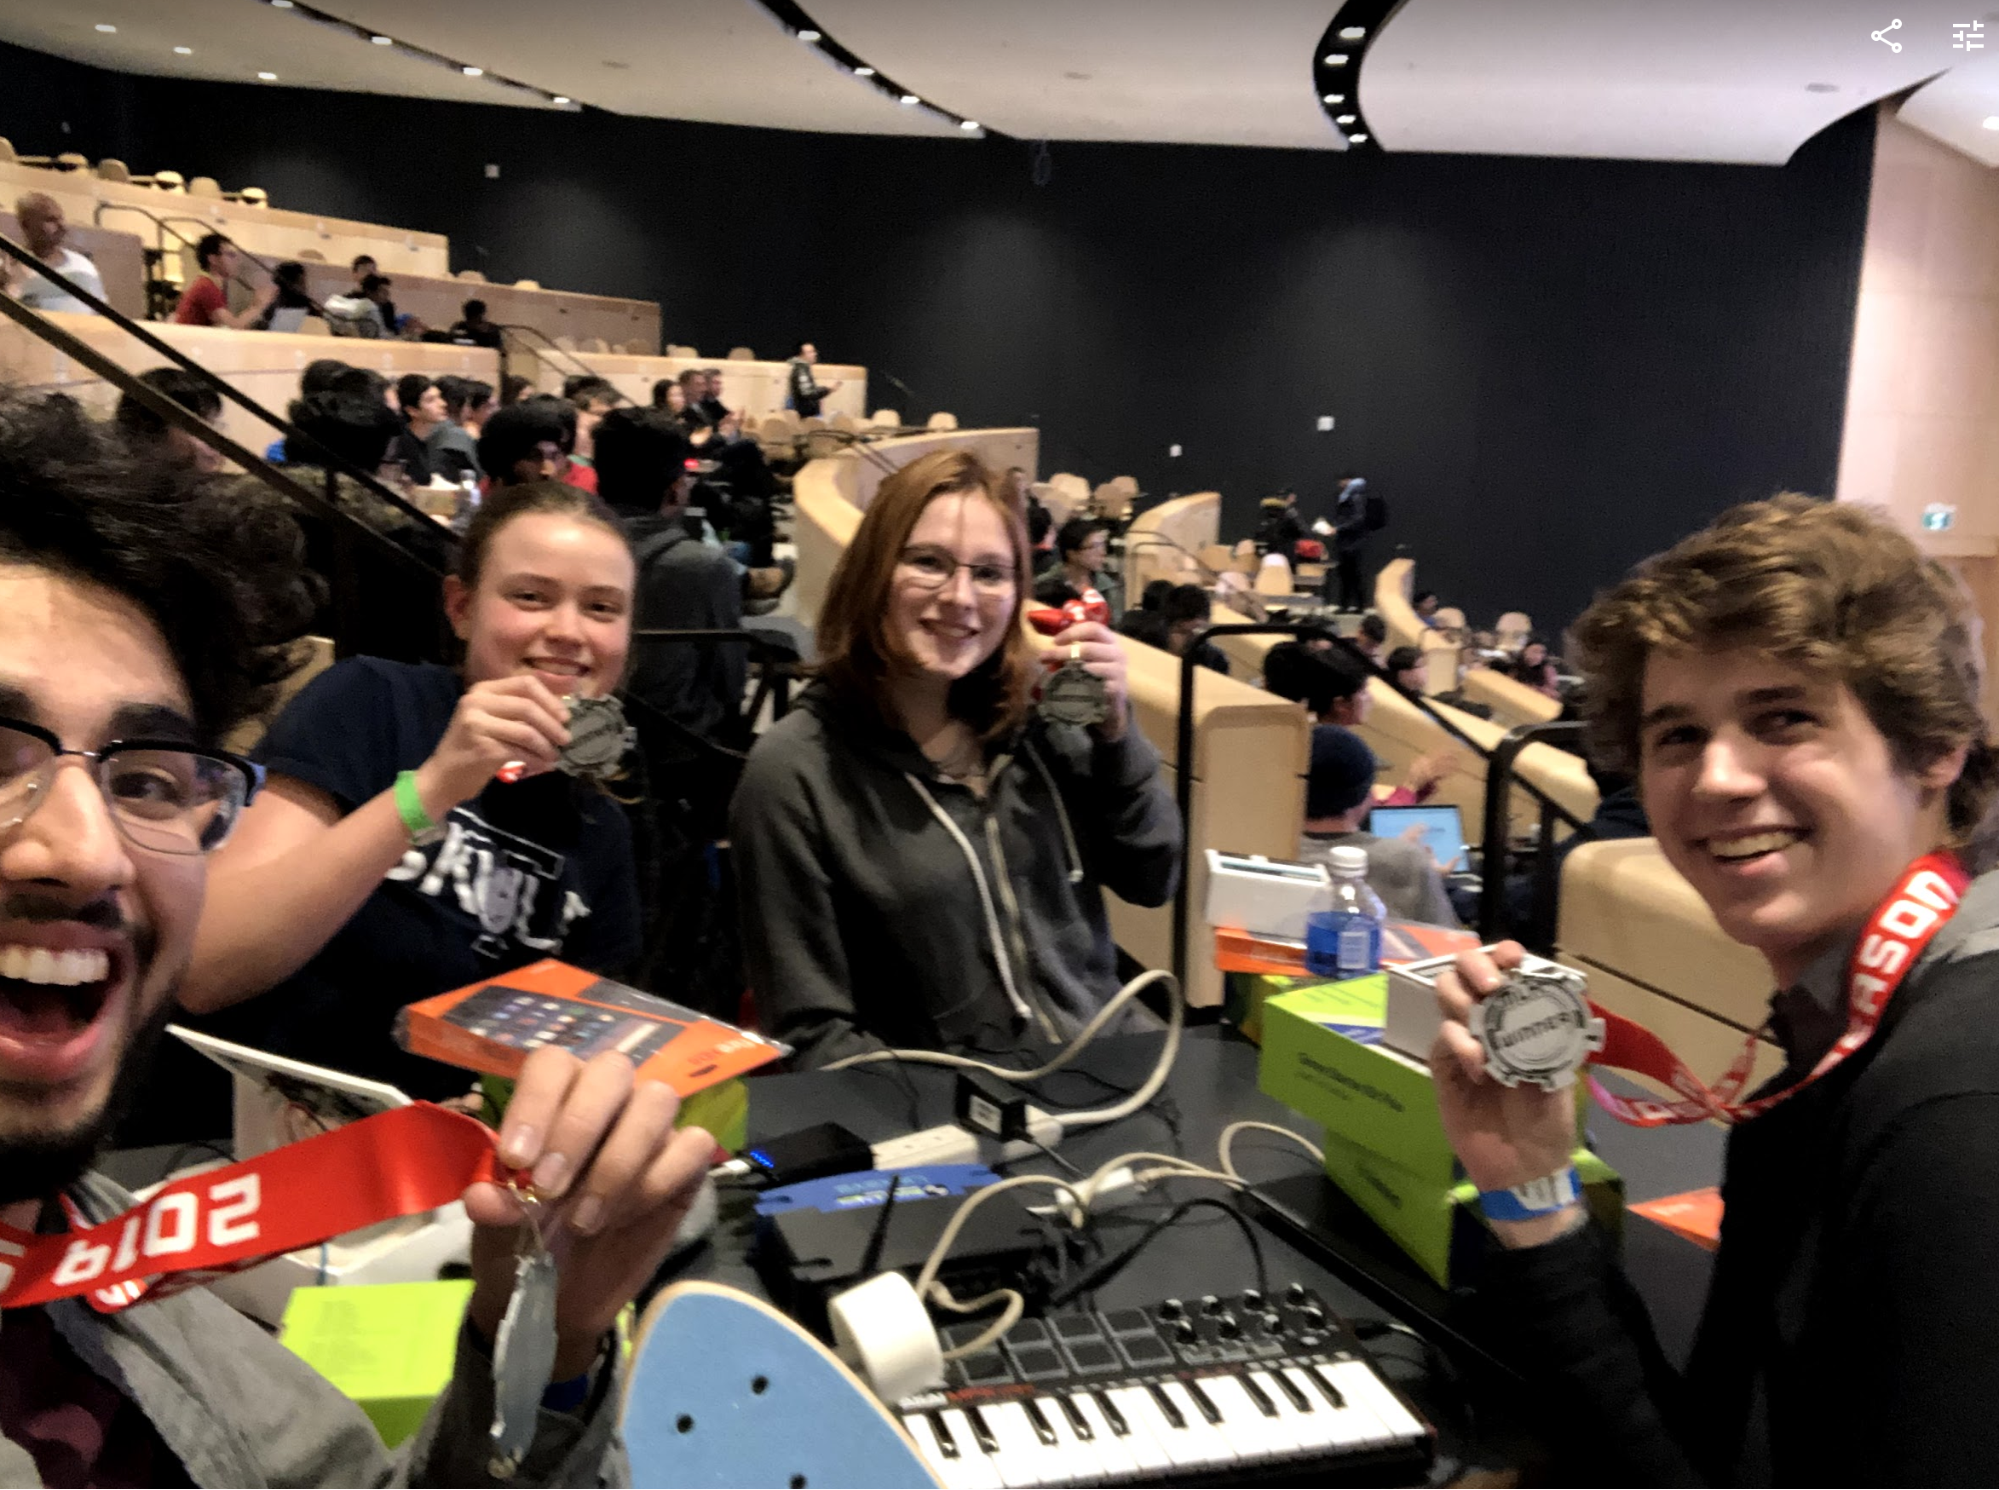
\includegraphics[width=0.4\textwidth]{img/image013.png}
\caption{Myself, Helen, Eli, and Adam with some of our prizes.}
\label{}
\end{figure}

\subsubsection{Holistic Review}

Helen playing the \textbf{devil’s advocate} (\ref{sec:devil}), as well as our use of the \textbf{MVP} (\ref{sec:MVP}) framework really drove our success in the hackathon. I also think that the importance of a solid team dynamic where each person trusts that the goal of each other person is to advance the project is import, along with a hierarchy of believability that each person can use to decide the degree to which they ought argue/accept each claim made by others in each domain of the project. For example, I readily gave into claims made by Adam when it came to networking because he had the most experience and expertise in the field and was therefore the most believable by far. Only if I were very sure of my reasoning and facts would I argue against his claims. Likewise, Eli was the most believable when it came to finding the best way for us to document and describe our process due to her clear competence in the field based on her past achievements and success in Praxis I. This sort of \textbf{believability-weighted decision making} (\ref{sec:believe}) is very important and valuable for making good decisions quickly and taking advantage of each person’s expertise on a given team.

I would also like to point out that, in the lecture in which he introduced the idea of an MVP in engineering design, Prof. Foster referenced our documentation for our hackathon project [1].

\subsection{Praxis II Firefighter RFP Implementation}
\label{sec:fire}
For our Praxis II project, Amy, Haochen, Yannis and I worked on the firefighters RFP that requested a solution to the lack of situational awareness in firefighting.

\subsubsection{Process}
We picked our RFP based on how interesting we thought it would be to work with the stated group and how interesting it would be to work on their problem. The most interesting one to us by far was working with firefighters on situational awareness. Firefighters have important and interesting jobs and situational awareness has a lot of potential to be improved by engineering and technology.

We began by scoping outward from the RFP because we felt that the requirement for our solution to help with both pathfinding and situational awareness really pushed toward a very specific type of situational awareness. After scoping out to just situational awareness, we did some research during the studio where we were supposed to be using “as many tools as possible” in order to diverge, much to chagrin of Professor Patricia Sheridan. We did this because we felt that we didn’t have enough of an understanding of the field from the RFP in order to properly diverge well. We thought our \textbf{pareto curve} (\ref{sec:pareto}) would be optimized if we were to research and then diverge. Once we felt we had enough research to do some effective diverging, we did some \textbf{multi-panel diverging} (\ref{sec:panel}) on the provided whiteboards. This was highly effective as it allowed us to \textbf{creatively recombine} various ideas, and we were able to literally take a step back from the board when we wanted to think in a more big-picture way and recombine ideas and take a step toward the board when we wanted to expand on one particular idea. We came up with three main ways to help the firefighters with situational awareness:

\begin{enumerate}
	\item Incorporating gas sensors into each firefighter’s suit to localize the fire/classify the type of fire.
	\item Incorporating physiological sensors into the firefighter’s suits to track the cardiovascular health of each firefighter over time. 
	\item Creating an optimized version of the entry control board to minimize human error.
\end{enumerate}

\begin{figure}[H]
\centering
\includegraphics[width=0.65\textwidth]{img/image014.png}
\caption{Our 4-panel breadth-first diverging setup. Note the activity at the intersections of the panels (this was soome of the most valuable in the process)}
\label{}
\end{figure}

\begin{figure}[H]
\centering
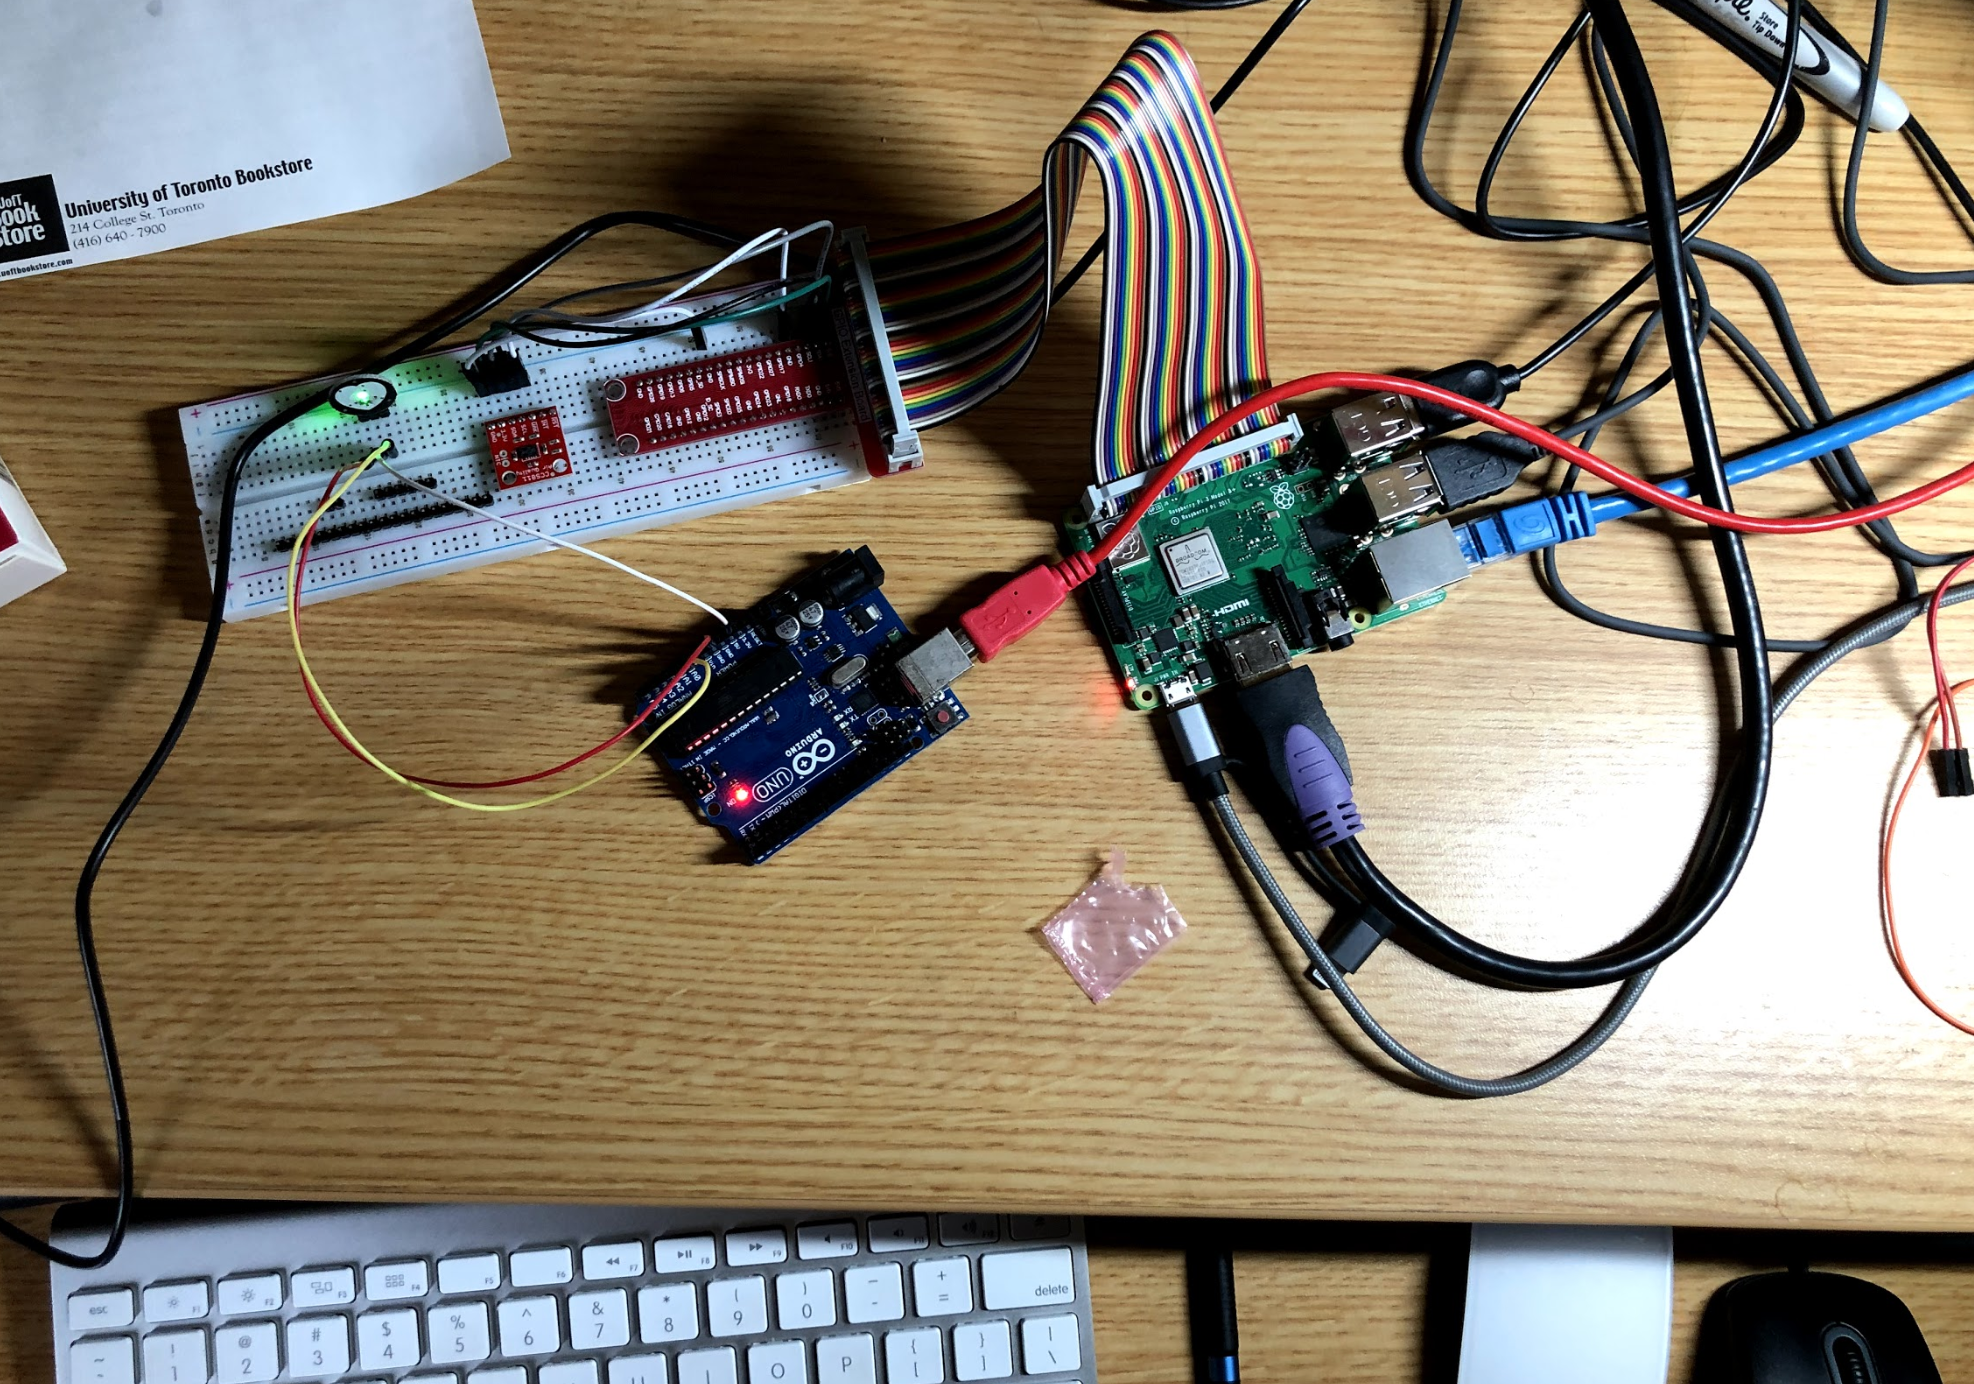
\includegraphics[width=0.65\textwidth]{img/image015.png}
\caption{Two of our resulting prototypes (gas and physiological sensors). These prototypes enabled us to be very sure of our choice to narrow down to entry control as our opportunity later on, and they existed thanks to our multi-panel diverging process}
\label{}
\end{figure}


When we had our first stakeholder interaction, they were fairly neutral when it came to the first two ideas, but they really liked the last idea about entry control. We created prototypes for each of them to get a better sense of what it would be like to actually implement them, and we presented our work at beta. We used \textbf{multi-vote} (\ref{sec:multi}) to narrow down to just the entry control board idea, and then used \textbf{sensitivity analysis} (\ref{sec:sense}) to confirm our choice. The multi-vote was very effective because the team’s interest and belief in the idea was an important quality for our project, and the sensitivity analysis enabled us to confirm that our mental models for evaluating the situation were consistent with a numerically encoded and agreed upon model of that same situation.

\begin{figure}[H]
\centering
\includegraphics[width=0.9\textwidth]{img/image016.png}
\caption{Our sensitivity analysis was highly effective in communicating why we made our decision to converge as well as in confirming our initial multi-vote and intuitive feelings on the matter.}
\label{}
\end{figure}

We had very positive feedback from our beta release, and it was at this point that we started on our more intense UI, cognitive load, and human error research to create our UI requirements model. Taking an idea from the famous Steve Jobs, a titan of design, we created our first rough prototype using the \textbf{shoshin} (\ref{sec:shoshin}) approach; we did no research beforehand and simply tried to generate what an entry control board ought to look like from first principles. It is a technique that essentially minimizes anchoring bias. Our shoshin prototype formed a great basis for our \textbf{iterative design} (\ref{sec:iter}) process. Our second prototype took a small step towards realism by incorporating some of our research.

\begin{figure}[H]
\centering
\includegraphics[width=0.8\textwidth]{img/image017.png}
\caption{The shoshin prototype was very quick and low-quality, but it we felt that it reduced our anchoring bias overall because our starting point for iteration was not affected by the status quo.}
\label{}
\end{figure}

At this point I began work on our third version that would hopefully be testable. It was a barebones version of an entry control board where every team and option was already hard-coded in. It functioned as an \textbf{MVP} (\ref{sec:MVP}) for our testing and showcase, as well as a proof of concept that the javascript library Angular.js could accomplish all the things we wanted from our digital entry control board.

\begin{figure}[H]
\centering
\includegraphics[width=0.8\textwidth]{img/image018.png}
\caption{A more testable prototype that still retains many elements from the shoshin version.}
\label{}
\end{figure}

From version 3.2-3.5, I iterated our design with the help of our UI requirements model, team feedback, and test user feedback. This process is what enabled us to move from a barebones, testable prototype to a fully functional prototype that had fantastic results with both validation with respect to our key metric of accuracy and with our stakeholder validation from real firefighters in station No. 315. The process also made it very easy to see what our next steps ought to be based on our requirements model and feedback from our stakeholders on our relatively highly actualized version.

\begin{figure}[H]
\centering
\includegraphics[width=0.7\textwidth]{img/image019.png}
\caption{Our line of iPads each running versions 3.1-3.5H on them was very effective in communicating the rigour of our process to the audience at showcase. Special thanks to Prof. Foster for offering the iPads.}
\label{}
\end{figure}

Meanwhile, we made a separate set of requirements for an improved analogue board to address more immediate issues from our stakeholder interactions. In order to make engineering sub-decisions, we used \textbf{pugh charts} (\ref{sec:pugh}) to decide on such elements as which clock to use, which board type, which pen type, and more.

\begin{figure}[H]
\centering
\includegraphics[width=0.9\textwidth]{img/image020.png}
\caption{The pugh charts were very effective in converting ratings matrices into more interpretable charts based on our criterion.}
\label{}
\end{figure}

\subsubsection{Holistic Review}
Though we haven’t received our grades for showcase yet, I believe that we will receive a high grade because of our well-implemented iterative design process and the quality of both testable and functional prototype that it produced. Our process allowed us to plug many potential holes in our design as well as to be aware of outlying holes in advance of our presentation.

\subsection{Recursive Self-Actualization}
\label{sec:self}
Since I was very young, I have had a firm belief that I am capable of accomplishing my goal of changing the world for the better in a significant way. I have always believed that was at least \textit{capable} of anything, I just needed time and resources.

However, for the first ~15 years of my life, you would have very few reasons to believe me. I was a lazy student with poor grades, didn’t have any interesting projects under my belt, and spent most of my time watching videos on the internet. I was pretty good at closeup card magic and speedcubing, but I wasn’t close to being the best in the world by any means.


\subsubsection{Process}
This disconnect between the reality I saw unfolding in my own life and the potential I felt so viscerally was a constant source of dissatisfaction, but it came to a head in March of 2015 while I was visiting my cousin in Texas. Feeling discouraged by my recent report card, my inability to speak Hindi, and my lack of self-actualization in general, I had the idea to do the following every week:

\begin{enumerate}
	\item List what went poorly that week/what I’m annoyed with/worried about (i.e. ‘bugs’)
	\item List how I am going to solve those problems (i.e. ‘fixes’)
	\item List what went well/what I’m happy with (i.e. ‘good things’)
\end{enumerate}

\begin{figure}[H]
\centering
\includegraphics[width=0.9\textwidth]{img/image021.png}
\caption{My very first weekly review. This process started out extremely simply, but the important thing was that it could be \textit{recursively} self-improving, which will be discussed at length below.}
\label{}
\end{figure}

My reasoning for starting this was as follows: \textit{If I want my life to improve, how I can I expect it to do so if I don’t have feedback loops built in at regular intervals? Since the feedback loops provided by life (i.e. report cards, new years, Diwali, etc.) clearly aren’t enough for me, I must create my own at more regular intervals.}

What I didn’t realize at the beginning was that this process could be \textbf{recursively self-improving}. Under the ‘bugs’ section, I may list a problem I see with the review system itself and attempt to fix it in the coming weeks. Therefore, in addition to being generally improving to myself, it is improving to itself. Now, my review system includes:

\begin{enumerate}
	\item General, journal like reflection on the week to prime myself for more analytical reflection.
	\item List the 20\% of things causing 80\% of what I’m dissatisfied with (i.e. ‘bugs’)
	\item List how I can solve/if I should solve these and make solving them as efficient as possible (i.e. ‘fixes’)
	\item List the 20\% of things causing 80\% of things I’m happy about (i.e. ‘good things’)
	\item Brainstorming of systematic errors I may be making in my life (Am I on the path upon which I want to be? What makes me think that? How has that changed (if at all) in this last week?)
\end{enumerate}

\begin{figure}[H]
\centering
\includegraphics[width=0.9\textwidth]{img/image022.png}
\caption{The layout for my last weekly review. I chose not to include the full text here because it includes several rather personal matters I would not like to share.}
\label{}
\end{figure}

I have continued to use this system every week (along with special reviews each month, semester, and year) for 4 years and 21 days as of writing this handbook. Since starting, my academics, extra-curricluar activities, hobbies, and overall self-actualization has improved dramatically and consistently.

\subsubsection{Validity as an Engineering Project}

This is a highly valid project for this assignment as it incorporates tools, models, frameworks such as recursive self-improvement, 80-20 analysis, and iterative design. By definition, “Engineers apply the knowledge of the mathematical and natural sciences (biological and physical), with judgment and creativity to develop ways to utilize the materials and forces of nature for the benefit of mankind.” [2]. In this case, I am using my knowledge of my life and the natural sciences (in addition to social sciences) with judgement and creativity to improve my life. The wikipedia definition for engineering fits this project even better:
\begin{quote}
Engineering is the application of knowledge in the form of science, mathematics, and empirical evidence, to the innovation, design, construction, operation and maintenance of structures, machines, materials, software, devices, systems, processes, and organizations. [3]
\end{quote}
I believe that this is a strong example of engineering, and that the techniques I continue to use in this are highly valid and applicable tools to other projects (especially those involving the optimization of qualitative, subjective systems that are subject to an unknown/immeasurable set of stimuli/conditions.


\section{Personal Design Process}


\begin{figure}[H]
\centering
\includegraphics[width=0.9\textwidth]{img/image024.png}
\caption{Red numbers indicate where each tool described in the tool section might be used. Decisions about which path to take from a given node are to be made by the team on a subjective basis, but can be informed by the description of process shown below.}
\label{}
\end{figure}

\subsection{Brief Description of Process}
\subsubsection{Central Path Justification}
\begin{enumerate}
	\item ‘Find Opportunity’ generally goes to ‘Research Opportunity’ because one must have ground to stand on when making arguments for the rest of the design process.
	\item ‘Research Opportunity’ generally goes to ‘Form Design Objectives’ because that begins the first step of forming proxy metrics and criteria.
	\item ‘Form Design Objectives’ generally goes to ‘Form Low Level Objectives, Metrics, and Criteria’ because more detailed proxies for goodness are often required for useful design.
	\item This leads to ‘Diverge’ and ‘Converge’ high-level alternatives because one now has the tools required to evaluate high-level alternatives in a system 1.5 way based on requirements model and research.
	\item This leads to ‘Divide and Conquer’ because this allows a team to go from a high-level design to a low-level, specified design quickly while maintaining rigour.
	\item ‘Divide and Conquer’ leads to the creation of the final product because at this point the team has a fully-specified design that only needs to be implemented.
\end{enumerate}

\subsubsection{Justification for Alternative Paths}

\begin{enumerate}
	\item Shoshin prototyping is a valid intermediate if the team believes it might be useful in the future (Shoshin can not be done after research as the anchoring bias has already set in).
	\item Researching the opportunity can lead to consulting with experts because it is highly likely that many opportunities I engage with will require far greater understanding than is feasible for me to assemble on my own during the anticipated time frame.
	\item Researching the opportunity can also lead to continuous argumentation because, if the team has a comprehensive enough understanding of the solution space and the other prerequisites for continuous argumentation (discussed in Tools section), they can skip the rest of the process and start with argumentation to rapidly optimize the solution.  
	\item Researching the opportunity can lead back to finding an opportunity if the opportunity is revealed to be flawed based on the research.
	\item Iteration can stem from diverging or converging because one only needs a single design to start iterating the design, and it is up to the team’s judgement whether the idea is good enough to start iterating.
	\item Iteration can go back and forth between automated and non-automated iteration because one’s models may or may not be numerical enough to be implemented well on a computer within the schedule of the project.
	\item Converging can lead back to diverging because one can converge to zero ideas.
	\item Converging can lead to continuous argumentation for the same reasons that research can lead to continuous argumentation. 
	\item Converging can lead to high-level prototyping because high-level prototypes can help with further understanding the high-level proposed design and in generating next steps for narrowing down the design.
	\item Converging can also lead to making an MVP because it an MVP is a great way to prove a concept is valid and feasible in the given timeframe.
	\item An MVP can lead to the creation of a final product because the idea is that an MVP is the core of a final product’s functionality. Adding features and testing is all that is necessary for going from an MVP to a final product.
\end{enumerate}

\subsection{Metadiscourse on Personal Design Process}
\begin{itemize}
	\item Pre-supposes University or GTA environment (e.g. “Consult Experts”)
	\item Assumes a team of 1-6 people because the projects described in this handbook have this size of team.
	\item This is a valid personal design process because it clearly draws from my experiences described in the Projects section and 
\end{itemize}





\section{Tools Index \label{Tools}}
\textit{Note: Unreferenced tools were created by me.}
\subsection{Multi-vote [4]}
\label{sec:multi}
\paragraph{Highlighted Project(s): } Praxis II Firefighter RFP Implementation \ref{sec:fire}
\paragraph{How it works: } 
Used for converging, especially when team interest, biases, etc. are to be considered in the decision.
\begin{itemize}
	\item Have each person in a ~4 person team select and rank their top 3 alternatives
	\item Add up scores for each idea.
	\item Select the top choice(s) to converge to or argue among the team and repeat.
\end{itemize}

\paragraph{Why it works for me: }
\begin{itemize}
	\item Argumentation enables me to better think through the decision if necessary and if there is disagreement.
	\item Allows people to play devil’s advocate.
	\item Increases efficiency (one of my values) by getting through decisions quickly.
\end{itemize}

\paragraph{Drawbacks: }
\begin{itemize}
	\item Weighs each person’s opinion evenly, going against the ‘believability weighted decision making’ principle.
	\item Therefore works better for evenly balanced teams/teams that are self-aware with respect to their levels of competence in relevant domains.
	\item Following blindly without proper understanding/discussion of each person’s view can lead to poor decisions that are skewed by a number of biases.
\end{itemize}

\subsection{How/wow/now matrix [5]}
\label{sec:how}
\paragraph{Highlighted Project(s): } UofT Consulting Association Engagemen (\ref{sec:UTCA})
\paragraph{How it works: } 
\begin{itemize}
\item Form a graph with axes {difficulty of implementation, expected value}
\item Plot (using system 1-1.5) each solution, feature, idea on the graph.
\item Cluster the following ideas:
\begin{itemize}
\item How = High difficulty, high value
\item Wow = Low difficulty, high value
\item Now = Low difficulty, low value
\end{itemize}
\end{itemize}

\paragraph{Why it works for me: }
I tend to lead my teams, and I need a way to prioritize who to put on which tasks when, and this helps a lot. As well, I enjoy representing my ideas to clients/stakeholders/those who are interested, and this helps communicate a hierarchy of ideas.

\paragraph{Drawbacks: }
It’s more of a tool to reveal what you think already about the ideas - not a tool to make novel decisions. It doesn’t do much to take care of your biases - if you are biased to {like, dislike} an idea, you will run into problems with ranking them too high/low in the axes.

\subsection{Solo to Group Brainstorming [6]}
\label{sec:solo}
\paragraph{Highlighted Project(s): } Praxis II Launcher
\paragraph{How it works: } 
Each person takes 1 < n < 5 minutes alone to brainstorm ideas for a given {opportunity, problem, objective, etc.}. The group then comes together to share their ideas and evaluate potential {connections, hierarchies, etc.}

\paragraph{Why it works for me: }
I value creativity, and this helps for more unique ideas to come forward. When brainstorming begins with everyone together, people quickly become anchored by the flow of the conversation. Thinking alone at first helps to preserve each person’s background and creative input to the process as a whole.


\paragraph{Drawbacks: }
\begin{itemize}
	\item Without proper research and understanding, brainstorming have useless outcomes.
	\item If a member is too overbearing, they can skew the results and mute others.
	\item If a member is too shy, they can detract from the discussion by not adding their ideas to the mix.
	\item Therefore, the team must be knowledgeable and comfortable with each other in order to fully leverage this technique.
\end{itemize}

\subsection{Multi-Panel Diverging}
\label{sec:panel}
\paragraph{Highlighted Project(s): } Praxis II Firefighter RFP Implementation (\ref{sec:fire})
\paragraph{How it works: }
\begin{itemize}
	\item Divide a board into panels/sections for each high-level {idea, opportunity, alternative, etc.}
	\item Have the team add detailed sub-{ideas, opportunities, alternatives} and details pertaining to them.
	\item Step closer to the board to expand things on the micro-scale
	\item Step away to look at a high-level overview and creatively recombing/diverge at the intersections of the panels.
\end{itemize}

\paragraph{Why it works for me: }
\begin{itemize}
\item I value creativity and this has helped with coming up with creative solutions.
\item It also allows for many people to work on the process at once. 
\item Once can literally step back to view the process at a high level AND at a low-level, increasing fluency/recording of ideas.
\end{itemize}

\paragraph{Drawbacks: }
\begin{itemize}
	\item Without proper research/prior understanding of the subject, it can have poor results.
	\item Too many panels can lead to sensory overload (greater than ~7, by experience)
	\item To address these, one must conduct enough research so the team has a comfortable understanding of the solution space, and they must have a proper number of dimensions in the {idea, opportunity, alternative} space (i.e. >7)
\end{itemize}

\subsection{Minimum Viable Product (MVP) [7]}
\label{sec:MVP}
\paragraph{Highlighted Project(s): } Play the Orchestra (\ref{sec:orch})
\paragraph{How it works: }
The minimum viable product is a version of the product that involves the minimum amount of work possible in order to communicate the important ideas in the product.

\paragraph{Why it works for me: }

\begin{itemize}
\item I value efficiency and practicality and I am biased to enjoy using my skills.
\item This allows me to do both.
\item It also enables a team to identify ideas/opportunities that are feasible within a given time frame based on the ease of implementation of the MVP.
\end{itemize}

\paragraph{Drawbacks: }
Does not make sense for all projects - very biased toward software/iterable projects with a clear dichotomy between core and optimal/extra functionalities. Therefore one must evaluate the predicted solution space to ensure that a good number of the possible solutions fit this criteria before using this tool.

\subsection{Continuous Argument}
\label{sec:argue}
\paragraph{Highlighted Project(s): } Praxis II Launcher (\ref{sec:launch})
\paragraph{How it works: }
A team continuously argues over why any number of alternatives are good. The team recombines the best aspects and filters down to the best ideas in order to arrive at a final solution.

\paragraph{Why it works for me: }
I find argumentation allows me to clarify and improve my mental models of any given situation. When my team and I have a strong grasp of the underlying concepts for the alternatives being considered, we all have a common ground to stand upon for making our arguments and optimizing our final solution.

\paragraph{Drawbacks: }
This only works well when the team shares a solid understanding of the underlying concepts AND are able to effectively communicate and argue their ideas pertaining to the alternatives. Therefore, one must ensure that the team is comfortable with each other and share a common understanding.

\subsection{Shoshin Prototyping [8]}
\label{sec:shoshin}
\paragraph{Highlighted Project(s): } Praxis II Firefighters RFP Implementation (\ref{sec:fire})
\paragraph{How it works: }
Shoshin is a buddhist concept that states that the inexperienced mind is more innovative and creative than the experienced one. It helps to minimizing a team’s anchoring bias. To implement a shoshin prototype, a team must not have engaged in significant research on the subject before hand. They generate a minimalist solution based on their first-principles understanding of the problem.

\paragraph{Why it works for me: }
I value the first-principles approach, and I believe in the power of iterative design. Shoshin prototypes can form a great basis for iterative design as they are relatively unaffected by anchoring bias.

\paragraph{Drawbacks: }
Shoshin prototypes can be completely useless if the team’s understanding of the opportunity is faulty (which is likely due to the purposeful lack of research). Furthermore, there is a strong chance that the team will miss a great idea that a reference design might incorporate. Therefore, shoshin prototypes must be used purposefully and be evaluated critically, and a team should always be willing to throw out the prototype.

\subsection{Extreme DfX [9]}
\label{sec:extreme}
\paragraph{Highlighted Project(s): } Praxis I Design - Smart Hat (\ref{sec:hat})
\paragraph{How it works: }
Making different alternatives to solve a problem, each of which takes one design objective to an extreme.

\paragraph{Why it works for me: }
I value open mindedness, and this approach enables one to open their mind to many ideas. It gives a group many design ideas to choose from, and can increase a group’s creativity by forcing them to think of methods of addressing a problem that they may not have otherwise.

\paragraph{Drawbacks: }
Depending on the number of design objectives, this can take a very long time. Group members that are highly concerned with time efficiency and direct progress may become frustrated with the seemingly roundabout way by which this method functions. Therefore, the group must be sufficiently open minded to (potentially) wasting time and having some absurd fun during the design process.

\subsection{Divide and Conquer}
\label{sec:conquer}
\paragraph{Highlighted Project(s): } Praxis I Design - Smart Hat (\ref{sec:hat})
\paragraph{How it works: }
After deciding on a high-level design, the team works to divide the design into many sub-decisions. The group then runs the design process like a fractal on the sub-decisions in order to generate a final detailed design.

\paragraph{Why it works for me: }
I value efficiency. Divide and conquer increases efficiency because, instead of running through the design process with many fully-fledged detailed design, it specifies to one high-level design and then runs the engineering design process on each sub decision.

\paragraph{Drawbacks: }
The team must be wary as to the level of rigour they use on each sub-design decision. In the worst case scenario, it can feel like doing 6+ full design projects. The team must learn to balance the importance of each sub-design decision with the amount of time/rigour allocated to it.

\subsection{Pugh Chart [10]}
\label{sec:pugh}
\paragraph{Highlighted Project(s): } Praxis II Firefighter RFP Implementation (\ref{sec:fire})
\paragraph{How it works: }
The team creates a ratings matrix for metrics or objectives from the requirements model and selects one design as a reference design. Plus signs are added where one design outperforms the reference, zeros for where they are equal, and negative signs where the reference outperforms the given design. Engineering arguments are made based on this in order to converge from the initial number of alternatives.

\paragraph{Why it works for me: }
It enables a team to more efficiently view and argue for why none design might outperform another (I value efficiency) while maintaining rigour. Makes it easier to remember how utility curves change the meaning of a rating’s matrix when comparing multiple alternatives.

\paragraph{Drawbacks: }
Ratings matrix take a long time to make, and pugh charts do to. It is tempting to blindly follow the sums of the columns to make a decision. Therefore the team must be wary as to how often they use pugh charts to compare alternatives.

\subsection{Sensitivity Analysis [11]}
\label{sec:sense}
\paragraph{Highlighted Project(s): } Praxis II Firefighter RFP Implementation (\ref{sec:fire})
\paragraph{How it works}
One adds up the columns of a pugh chart for metrics/objectives of each alternative. Observe how the top ranked alternative(s) change as the weight of each metric/objective is tuned.

Sensitivity analysis can also apply to other decision making tools that can be made more numerical.

\paragraph{Why it works for me: }
It allows me to \textbf{triangulate} (\ref{sec:tri}) our engineering argumentation/design process and make sure that there isn’t something that we are missing in our numerical model of the decision or in our mental model of the decision.

\paragraph{Drawbacks: }
If followed blindly, teams can easily be misled by the collective error of approximated weight/ranking values. Therefore, teams must use this in conjunction with other decision making techniques in order to extract maximal benefit.

\subsection{Devil’s Advocate [12]}
\label{sec:devil}
\paragraph{Highlighted Project(s): } Play the Orchestra (\ref{sec:orch})

\paragraph{How it works: }
A person will disagree with the consensus of the team for the sake of disagreeing in order to reveal potential flaws in the reasoning of the team.

\paragraph{Why it works for me: }
Creative arguments must be made, and it is an efficient way to find holes in the team’s argument/process before they become too fixed. I value creativity and efficiency.

\paragraph{Drawbacks: }
If the team members are not comfortable with each other/open, this can cause resentment between members. If the devil’s advocate doesn’t know when to stop or becomes too invested in disagreeing, they can inhibit the progress of the team. Therefore, the team must first be comfortable enough and be self-aware enough to not harm the progress of the team by playing devil’s advocate.

\subsection{80-20 Risk Management Analysis}
\paragraph{Highlighted Project(s): } Recursive Self-Actualization (\ref{sec:self})

\paragraph{How it works: }
When trying to accomplish something, try to determine what 20\% of possible actions that will push that thing to fruition will cause 80\% of the progress.

\paragraph{Why it works for me: }
This increases efficiency and has helped me to clarify my mental model of complex, subjective matters that I need to rapidly optimize.

\paragraph{Drawbacks: }
It can be difficult to adequately determine which exactly 20\% of things will cause exactly 80\% of the progress - these are just guideline numbers to start the process of optimization, and the user of this must realize that.

\subsection{Pareto Curve Optimization [14]}
\label{sec:pareto}
\paragraph{Highlighted Project(s): } CIV102 Bridge Project (\ref{sec:bridge})

\paragraph{How it works: }
Tool to talk about your rate of progress on a given activity (e.g. “our pareto curve is great because we are making fast progress because of {something}”). Optimizing this is a very solid way to make fast progress in time-sensitive assignments.


\paragraph{Why it works for me: }
I value open mindedness and the rate of progress and optimizing that rate is an important thing to discuss in a team. In order to be open minded about ideas pertaining to this rate of progress, common vocabulary must be implemented, and this helps with communication.


\paragraph{Drawbacks: }
It must be clear what variable the pareto curve is with respect to: is it progress towards finishing the requirements model, or is it actually the final design? One can optimize their pareto curve for one thing while neglecting others, so being conscious of which variable the pareto curve relates to is paramount to success.



\subsection{Expected Value Calculations}
\label{sec:value}
\paragraph{Highlighted Project(s): } CIV102 Bridge Project (\ref{sec:bridge})

\paragraph{How it works: }
In order to calculate the expected value of an action, they multiply the projected reward from the successful outcome of the action by the chance of success in that action. Actions with higher expected values are to be prioritized.

\paragraph{Why it works for me: }
It helps with quantifying efficiency (one of my values). It is also a great tool for understanding the benefit of a giiven action action and minimizing sunk cost fallacy/bias.

\paragraph{Drawbacks: }
It is difficult to find a good proxy for ‘value’. Disconnect with respect to the projected ‘value’ of an action must be addressed quickly to ensure that one had common ground with their teammates.

\subsection{Triangulation}
\label{sec:tri}
\paragraph{Highlighted Project(s): } UofT Consulting Association Engagement (\ref{sec:UTCA})

\paragraph{How it works: }
Substantiating claims by referencing multiple sources.

\paragraph{Why it works for me: }
I have found that it improves logos, ethos, especially with assessors in 100-level university courses and high school courses. It also makes the team more sure about the claims made in their argument.

\paragraph{Drawbacks: }
Takes significant time, so the team must prioritize the most important claims that should be substantiated first.


\subsection{Believability-weighted decision making [17]}
\label{sec:believe}
\paragraph{Highlighted Project(s): } Play the Orchestra (\ref{sec:orch})

\paragraph{How it works: }
When making a decision with multiple people’s inputs, one must value the input of each person proportionally to their believability.

\paragraph{Why it works for me: }
In a university/GTA environment, there are many people willing to input their ideas. As well, in the Engsci class, there is a wide variety skill sets and levels of experience. Therefore, one ought to weight the believability of each person giving advice in order to make the most of a team, especially one made of Engsci’s.


\paragraph{Drawbacks: }
Assigning believability requires one to understand the field and do proper research on each person who’s input has an effect on the decision. As well, group dynamics can be harmed if a team member feels that they don’t have believability in any relevant field. One must be careful of how they go about publicizing how believable a person is.


\subsection{Iterative design [18]}
\label{sec:iter}
\paragraph{Highlighted Project(s): } Praxis II Firefighter RFP Implementation (\ref{sec:fire})

\paragraph{How it works: }
Changing a design relatively small amounts at a time, making changes based on feedback from {requirements model, user feedback, team feedback, stakeholder feedback}.

\paragraph{Why it works for me: }
I appreciate the rigour this applies and the holes in the design that it helps to fix/bring up/address.

\paragraph{Drawbacks: }
Takes time, only applicable when the high-level design has been locked in. If done too early, it can make people experience the sunk cost fallacy - it takes a lot of effort to iterate, and a team feels locked into the high-level design.

\subsection{Rapid, automated iterative design [19]}
\label{sec:automated}
\paragraph{Highlighted Project(s): } CIV102 Bridge Project (\ref{sec:bridge})

\paragraph{How it works: }
Coding a model for the high-level design into a computer and having it optimizing using {genetic algorithm, gradient descent, etc.}.

\paragraph{Why it works for me: }
It enables me to leverage my skills to be more efficient (I value both of those things).

\paragraph{Drawbacks: }
Only applicable when codable models for the system are representative of the “goodness” of the products. It is also a high risk, high reward scenario - coding tends to take a long time, one must have a inkling that the opportunity fits well with it.







\section{Source Extracts}
[1] Foster, Jason; Irish, Robert. (2019). Lecture 18 [Lecture slides]. Retrieved from \url{https://courses.engsci.utoronto.ca/esc102/}. [Accessed: 15-Apr-19].

[2] “About IAENG,” Welcome to IAENG (International Association of Engineers)! [Online]. Available: \url{http://www.iaeng.org/about_IAENG.html}. [Accessed: 15-Apr-2019].

[3] “Engineering,” Wikipedia, 14-Apr-2019. [Online]. Available: \url{https://en.wikipedia.org/wiki/Engineering}. [Accessed: 15-Apr-2019].

[4] N. R. Tague, The Quality Toolbox. Milwaukee, WI: ASQ Quality Press, 2009.

[5] “Now-Wow-How-Matrix.” Interaction Design Foundation.

[6] Foster, Jason; Irish, Robert. (2018). Lecture 2 [Lecture slides]. Retrieved from \url{https://courses.engsci.utoronto.ca/esc101/}. [Accessed: 15-Apr-19].

[7] Foster, Jason; Irish, Robert. (2019). Lecture 26 [Lecture slides]. Retrieved from \url{https://courses.engsci.utoronto.ca/esc102/}. [Accessed: 15-Apr-19].

[8] W. Isaacson, Steve Jobs. New York: Simon \& Schuster Paperbacks, 2013.

[9] Foster, Jason; Irish, Robert. (2018). Lecture 7 [Lecture slides]. Retrieved from \url{https://courses.engsci.utoronto.ca/esc101/}. [Accessed: 15-Apr-19].

[10] Foster, Jason; Irish, Robert. (2018). Lecture 17 [Lecture slides]. Retrieved from \url{https://courses.engsci.utoronto.ca/esc101/}. [Accessed: 15-Apr-19].

[11] Foster, Jason; Irish, Robert. (2019). Lecture 25 [Lecture slides]. Retrieved from \url{https://courses.engsci.utoronto.ca/esc102/}. [Accessed: 15-Apr-19].

[12] “Devil,” Merriam-Webster. [Online]. Available: \url{https://www.merriam-webster.com/dictionary/devilsadvocate}. [Accessed: 15-Apr-2019].

[13] T. Ferriss, “How to Finally Play the Guitar: 80/20 Guitar and Minimalist Music,” The Tim Ferriss Show, 11-Dec-2012.

[14] Foster, Jason; Irish, Robert. (2018). Lecture 29 [Lecture slides]. Retrieved from \url{https://courses.engsci.utoronto.ca/esc101/}. [Accessed: 15-Apr-19].

[15] J. Schrum, “Expected Values,” in Reinforcement Learning 1, 06-Aug-2015.

[16] Foster, Jason; Irish, Robert. (2018). Lecture 13 [Lecture slides]. Retrieved from \url{https://courses.engsci.utoronto.ca/esc101/}. [Accessed: 15-Apr-19].

[17] R. Dalio, Principles life and work. New York: Simon and Schuster, 2017.

[18] Foster, Jason; Irish, Robert. (2019). Lecture 18 [Lecture slides]. Retrieved from \url{https://courses.engsci.utoronto.ca/esc102/}. [Accessed: 15-Apr-19].

[19] Foster, Jason; Irish, Robert. (2018). Lecture 2 [Lecture slides]. Retrieved from \url{https://courses.engsci.utoronto.ca/esc101/}. [Accessed: 15-Apr-19].


























\end{document}
